%% Standalone source for Figure 2 -- specification-level condition means.
%% GENERATED by research/generate_revision_figures.py from the operative analysis
%% (results-checks.json, validated against analysis-results.json). Do not hand-edit;
%% re-run the script. Compile with tectonic/pdflatex -> fig2-perspec-means.pdf.
\documentclass[border=4pt]{standalone}
\usepackage{pgfplots}
\pgfplotsset{compat=1.18}
\begin{document}
  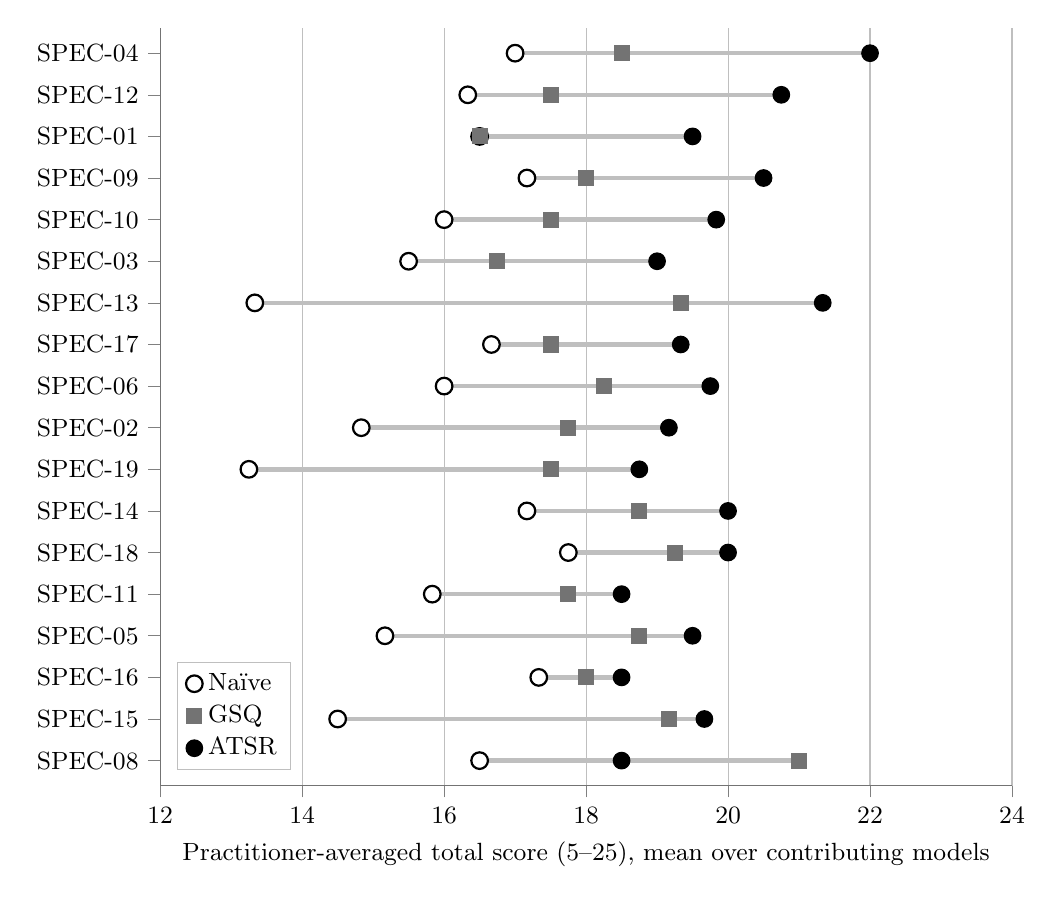
\begin{tikzpicture}
    \begin{axis}[
      width=12.4cm,
      height=11.2cm,
      xmin=12, xmax=24,
      xtick={12,14,...,24},
      xlabel={Practitioner-averaged total score (5--25), mean over contributing models},
      xlabel style={font=\small},
      xticklabel style={font=\small},
      ymin=0.4, ymax=18.6,
      ytick={1,...,18},
      yticklabels={{SPEC-08},{SPEC-15},{SPEC-16},{SPEC-05},{SPEC-11},{SPEC-18},{SPEC-14},{SPEC-19},{SPEC-02},{SPEC-06},{SPEC-17},{SPEC-13},{SPEC-03},{SPEC-10},{SPEC-09},{SPEC-01},{SPEC-12},{SPEC-04}},
      yticklabel style={font=\small},
      y dir=normal,
      xmajorgrids=true,
      grid style={black!25, line width=0.4pt},
      tick align=outside,
      axis line style={black!55},
      axis x line*=bottom,
      axis y line*=left,
      legend style={
        at={(0.02,0.02)},
        anchor=south west,
        font=\small,
        draw=black!25,
        fill=white,
        legend columns=1,
      },
      legend cell align=left,
      clip=false,
    ]
      \draw[black!25, line width=1.6pt] (axis cs:17.000000,18) -- (axis cs:22.000000,18);
      \draw[black!25, line width=1.6pt] (axis cs:16.333333,17) -- (axis cs:20.750000,17);
      \draw[black!25, line width=1.6pt] (axis cs:16.500000,16) -- (axis cs:19.500000,16);
      \draw[black!25, line width=1.6pt] (axis cs:17.166667,15) -- (axis cs:20.500000,15);
      \draw[black!25, line width=1.6pt] (axis cs:16.000000,14) -- (axis cs:19.833333,14);
      \draw[black!25, line width=1.6pt] (axis cs:15.500000,13) -- (axis cs:19.000000,13);
      \draw[black!25, line width=1.6pt] (axis cs:13.333333,12) -- (axis cs:21.333333,12);
      \draw[black!25, line width=1.6pt] (axis cs:16.666667,11) -- (axis cs:19.333333,11);
      \draw[black!25, line width=1.6pt] (axis cs:16.000000,10) -- (axis cs:19.750000,10);
      \draw[black!25, line width=1.6pt] (axis cs:14.833333,9) -- (axis cs:19.166667,9);
      \draw[black!25, line width=1.6pt] (axis cs:13.250000,8) -- (axis cs:18.750000,8);
      \draw[black!25, line width=1.6pt] (axis cs:17.166667,7) -- (axis cs:20.000000,7);
      \draw[black!25, line width=1.6pt] (axis cs:17.750000,6) -- (axis cs:20.000000,6);
      \draw[black!25, line width=1.6pt] (axis cs:15.833333,5) -- (axis cs:18.500000,5);
      \draw[black!25, line width=1.6pt] (axis cs:15.166667,4) -- (axis cs:19.500000,4);
      \draw[black!25, line width=1.6pt] (axis cs:17.333333,3) -- (axis cs:18.500000,3);
      \draw[black!25, line width=1.6pt] (axis cs:14.500000,2) -- (axis cs:19.666667,2);
      \draw[black!25, line width=1.6pt] (axis cs:16.500000,1) -- (axis cs:21.000000,1);
      %% Naive: open circle
      \addplot[only marks, mark=*, mark size=3pt, mark options={fill=white, draw=black, line width=0.8pt}]
        coordinates { (17.000000,18) (16.333333,17) (16.500000,16) (17.166667,15) (16.000000,14) (15.500000,13) (13.333333,12) (16.666667,11) (16.000000,10) (14.833333,9) (13.250000,8) (17.166667,7) (17.750000,6) (15.833333,5) (15.166667,4) (17.333333,3) (14.500000,2) (16.500000,1) };
      \addlegendentry{Na\"ive}
      %% GSQ: mid-gray square
      \addplot[only marks, mark=square*, mark size=2.7pt, mark options={fill=black!55, draw=black!55}]
        coordinates { (18.500000,18) (17.500000,17) (16.500000,16) (18.000000,15) (17.500000,14) (16.750000,13) (19.333333,12) (17.500000,11) (18.250000,10) (17.750000,9) (17.500000,8) (18.750000,7) (19.250000,6) (17.750000,5) (18.750000,4) (18.000000,3) (19.166667,2) (21.000000,1) };
      \addlegendentry{GSQ}
      %% ATSR: filled black circle
      \addplot[only marks, mark=*, mark size=3pt, mark options={fill=black, draw=black}]
        coordinates { (22.000000,18) (20.750000,17) (19.500000,16) (20.500000,15) (19.833333,14) (19.000000,13) (21.333333,12) (19.333333,11) (19.750000,10) (19.166667,9) (18.750000,8) (20.000000,7) (20.000000,6) (18.500000,5) (19.500000,4) (18.500000,3) (19.666667,2) (18.500000,1) };
      \addlegendentry{ATSR}
    \end{axis}
  \end{tikzpicture}
\end{document}
